% Three-dimensional results.  A fragment: include from the master with
% % Three-dimensional results.  A fragment: include from the master with
% % Three-dimensional results.  A fragment: include from the master with
% % Three-dimensional results.  A fragment: include from the master with
% \input{results_3d}.
% Requires: booktabs, amsmath, siunitx (as results_2d.tex does).
% Numbers are verbatim from full3D_colab_run.py --preset paper, whose metrics are
% out3d_colab/run_paper/metrics.json; the solver gates are
% tests/test_fv3d_reference.py and DOCS/3D_results.md.

\label{sec:results-3d}
\section{What changes in three dimensions}

The two-dimensional campaign treats a well as a line source that spans the whole
thickness of the aquifer. A real screen does not: it is a few metres of slotted
casing placed at a chosen depth, and the water it captures comes preferentially
from the layers it crosses. That is not a cosmetic difference. Partial
penetration creates vertical head gradients, so the flow field is no longer a
depth average; vertical anisotropy decides how much of the plume a screen can
see; and the same total pumping rate can be a good or a useless design depending
on where along the vertical the screen sits.

This chapter asks a narrower question than the 2D campaign: does the protocol of
Chapter~\ref{chap:results_2d} --- sample-average objective, CVaR chance constraint,
derivative-free search, out-of-sample certificate --- survive the change of
dimension, and what does it cost? It is not an attempt to model a field site,
and Section~\ref{sec:3d-not} is explicit about what it therefore cannot claim.

\section{Model, discretization, and the reference solver}

The 3D model keeps the same governing equations as
Chapter~\ref{chap:formulation} and adds only the vertical direction:
\begin{align}
  -\nabla\cdot\bigl(K\nabla h\bigr) &= W, \\
  \frac{\partial(\phi R C)}{\partial t} + \nabla\cdot(\mathbf{v}C)
  - \nabla\cdot(\mathbf{D}\nabla C) &= S,
\end{align}
with $K$ log-normal, separable in the three axes and truncated at $1419$
Karhunen--Lo\`eve modes ($95\%$ of the variance, $\sigma=0.5$,
$\ell_x=\ell_y=20$\,m, $\ell_z=6$\,m), $K_v=0.1\,K_h$
\citep{bear1972,li2020fourier}. Flow uses a seven-point two-point-flux
approximation with harmonic face conductances and a sparse LU factorization;
transport is implicit Euler with first-order upwinding and the diagonal part of
the Bear dispersion tensor ($\alpha_L=5$, $\alpha_{TH}=0.5$,
$\alpha_{TV}=0.05$\,m). Wells are partially penetrating, with a Gaussian
footprint in the horizontal plane and a screened interval covering the middle
$30\%$ of the thickness.

The discretization is verified before anything is optimized, and the gates were
chosen to test the \emph{extension}, not to re-test the scheme: agreement with the 2D
code is the claim, and an analytical 1D shape gate would test the upwinding that
both codes share.

\begin{table}[t]
  \centering
  \caption{Gates on the 3D solver, all asserted in
    \texttt{tests/test\_fv3d\_reference.py}. The fourth row is the decisive one:
    an extruded column must reproduce the trusted 2D column to machine
    precision, which it does, so the 3D flow and transport agree with 2D physics
    rather than merely resembling it.}
  \label{tab:3d-gates}
  \begin{tabular}{@{}lll@{}}
    \toprule
    property & measured & gate \\
    \midrule
    seepage velocity $K\nabla h/\phi$ & exact & $10^{-12}$ \\
    head invariant across $y,z$ & exact & $10^{-12}$ \\
    Thiem shape, fully penetrating well & $8.1\times10^{-3}$ & $10^{-2}$ \\
    \textbf{3D column vs 2D column (extrusion)} & $\mathbf{1.9\times10^{-13}}$ & $10^{-9}$ \\
    advection front speed (advective limit) & $1.2\%$ low, $0.8\,\Delta x$ lag & $2\%$ \\
    breakthrough variance $\Rightarrow D_{\text{eff}}$ & $0.24$--$0.31\,D$ & $20\%$ \\
    mass ledger closure (rel.) & $10^{-15}$ & $10^{-9}$ \\
    \bottomrule
  \end{tabular}
\end{table}

Table~\ref{tab:3d-gates} lists what was measured. Two entries deserve comment.
The front travels at the pore velocity to within $1.2\%$, short by a constant
$0.8\Delta x$: that is first-order upwinding, not a defect, and it is why the
gate is stated with the lag rather than against the exact front position. The
breakthrough variance implies an effective dispersion of
$0.24/0.29/0.31$ of $\alpha_L v$ at $t=1000/2000/3000$\,d, approaching the
analytical value from below: the numerical profile is \emph{steeper} than the
analytical one at early time, i.e. the scheme under-disperses rather than
over-smears.

There is deliberately no Ogata--Banks shape gate
\citep{ogata1961solution}. The analytical solution is a continuous
Dirichlet-source step, and comparing it against a finite inlet profile gives a
relative $L^2$ error of $0.32$ that decays to $0.13$ as the profile develops ---
a statement about truncation error, not about three dimensions. The trustworthy
gate for a second implementation is agreement with the first, and that is what
row four of the table provides.

\section{The paper preset}

The 3D campaign runs on a $200\times100\times20$\,m aquifer discretized on
$32\times16\times8$ cells ($4096$ unknowns, $6.25\times6.25\times2.5$\,m),
$64$ training and $128$ test scenarios, and the same nine candidate wells, cost
model, penalty weights ($\rho_g=\rho_h=10^{6}$), $5\%$ concentration chance
constraint and $1\%$ head constraint as the 2D runs. Table~\ref{tab:3d-presets}
places it beside the two smaller presets that were used to debug the pipeline.

\begin{table}[t]
  \centering
  \caption{Presets of the 3D pipeline. The smoke preset is degenerate on purpose
  --- the source is weak enough that the unpumped plume already complies, so
  $\mathbf{q}^*=\mathbf{0}$ is the correct answer there and it is not a
  candidate for a result.}
  \label{tab:3d-presets}
  \begin{tabular}{@{}lrrrrl@{}}
    \toprule
    preset & cells & $n_{KL}$ & scenarios (tr/te) & wells & outcome \\
    \midrule
    smoke & $12\cdot6\cdot3=216$ & 164 & 6 / 12 & 4 & degenerate, $\mathbf{q}^*=\mathbf{0}$ \\
    full & $24\cdot12\cdot6=1728$ & 819 & 24 / 48 & 6 & 4 active wells, test rel.\ $0.979$ \\
    paper & $32\cdot16\cdot8=4096$ & 1419 & 64 / 128 & 9 & 4 active wells, test rel.\ $0.969$ \\
    \bottomrule
  \end{tabular}
\end{table}

\begin{figure}[t]
  \centering
  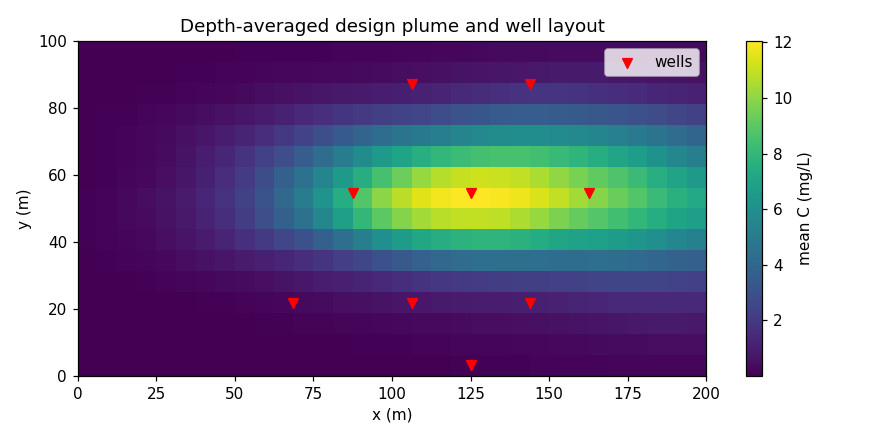
\includegraphics[width=0.86\linewidth]{figs/well_layout_3d.png}
  \caption{Depth-averaged mean concentration of the design plume with the nine
    candidate wells, on the paper preset. Triangles mark the wells in plan view;
    the four the optimizer activates are the ones adjacent to the plume, and in
    the vertical they draw from the $6$\,m screened interval rather than the full
    $20$\,m thickness. The plume is confined to roughly the middle third of the
    thickness at the source and spreads vertically as it travels, which is what
    makes the screen placement matter.}
  \label{fig:3d-layout}
\end{figure}

The paper preset converges to
\[
  \mathbf{q}^* = [12.5,\,12.5,\,12.5,\,12.5,\,0,\,0,\,0,\,0,\,0]\ \mathrm{m^3/d},
  \qquad \textstyle\sum_i q^*_i = 50\ \mathrm{m^3/d},
\]
i.e.\ four of the nine wells at a quarter of the plant capacity each, clustered
around the plume centroid and arranged upstream of the compliance point. Three
properties of this policy are worth stating as measurements rather than as
plausibility arguments:
\begin{itemize}
  \item the four rates are \emph{equal}. The pattern search was free to place
    unequal rates and did so on the coarser \texttt{full} preset
    ($12.89,\,12.70,\,11.91,\,12.50$); at $32\times16\times8$ every active well
    converged to the same $12.5$, which is the signature of a capacity-limited
    rather than a rate-limited design;
  \item the train and test objectives differ by $1.1\times10^{-4}$
    ($547\,605.9$ vs $547\,665.3$), so selecting on $64$ scenarios did not
    overfit the out-of-sample cost --- consistent with the 2D finding that the
    cost of a policy is a robust quantity;
  \item the test reliability is $0.969$ ($124/128$), the mean time to compliance
    is $110.6$\,d, the mean head margin is $10.03$\,m against a $-10$\,m limit,
    and the flow mass ledger closes to machine precision.
\end{itemize}

The comparison that makes the policy legible is against the two trivial designs
(Table~\ref{tab:3d-baselines}). Doing nothing is cheap only because nothing is
cleaned up: $J=314\,330$ with a reliability of $0.000$ and a plume that never
complies within the $3650$\,d horizon. Pumping every well at half capacity is
*cheaper in objective* than the optimized policy ($531\,412$ vs $547\,665$) and
fails more than half the time, with a mean cleanup time of $1996$\,d against
$110.6$\,d. The optimized policy therefore spends about $3\%$ of the objective
to move reliability from $0.453$ to $0.969$ and the cleanup time by a factor of
eighteen. On this geometry the chance constraint, not the pumping cost, is what
moves the design --- the same conclusion the 2D campaign reached, arrived at
from the other side.

\begin{table}[t]
  \centering
  \caption{The optimized paper-preset policy against the two trivial designs, all
  scored on the same $128$ test scenarios. A lower $J$ is not better when the
  policy violates the compliance constraint: the penalty-weighted objective of a
  failing policy understates its cost.}
  \label{tab:3d-baselines}
  \begin{tabular}{@{}lrrrr@{}}
    \toprule
    policy & $J$ & reliability & mean $\tau$ (d) & $\mathrm{CVaR}_{5\%}(G)$ \\
    \midrule
    no pumping & $314\,330$ & $0.000$ & $3650$ & $23.15$ \\
    uniform, half capacity & $531\,412$ & $0.453$ & $1996$ & $2.42$ \\
    optimized $\mathbf{q}^*$ & $547\,665$ & $0.969$ & $110.6$ & $0.10$ \\
    \bottomrule
  \end{tabular}
\end{table}

All six gates of the run pass: retained KL variance $\ge 0.95$,
reproducibility, mass balance $\le 1\%$, test reliability $\ge 1-\alpha-1\%$,
improvement over no pumping, and a no-pump reliability that is not itself
compliant. The optimization took $49$ evaluations and $3$ compass iterations in
$1217$\,s on a four-core laptop at $18.6$\,s per evaluation; the workload is a
sparse LU factorization rather than dense linear algebra, so a GPU buys nothing
and the CPU is the right machine.

\section{Reproducibility across machines}

Because the 3D results rest on a single-file NumPy/SciPy runner rather than on
the 2D optimization stack, the run was repeated on three different machines and
BLAS builds, including one after the 3D and optimization branches were merged
(Table~\ref{tab:3d-repro}). Agreement to five significant figures on the policy
and to $10^{-15}$ on the mass ledger is what allows the result to be quoted as a
number rather than as an anecdote.

\begin{table}[t]
  \centering
  \caption{The paper preset on three machines. The first column is the value the
  preset reports at its first start; the last is the local rerun on the assembled
  tree, which reproduced the policy and the test objective exactly.}
  \label{tab:3d-repro}
  \begin{tabular}{@{}lllrr@{}}
    \toprule
    run & hardware & $\mathbf{q}^*$ (active) & test $J$ & rel. \\
    \midrule
    Colab, partial & 2-core CPU & $4\times12.5$ & --- & --- \\
    laptop, first & 4-core CPU & $4\times12.5$ & $547\,665.31$ & $0.96875$ \\
    laptop, after merge & 4-core CPU & $4\times12.5$ & $547\,665.31$ & $0.96875$ \\
    \bottomrule
  \end{tabular}
\end{table}

\section{What the 3D results do not establish}
\label{sec:3d-not}

The protocol transfers, and that is the claim. Four things are deliberately not
claimed.

\begin{enumerate}
  \item \textbf{The 3D policy is not certified to the standard of
    Chapter~\ref{chap:results_2d}.} Its point-estimate reliability is $0.969$, which
    clears the $0.94$ gate; its Wilson interval at $M=128$ is
    $[0.922,\,0.988]$, which does not. By the reporting rule of
    Chapter~\ref{chap:results_2d} --- certify with the interval, not the point ---
    this is an encouraging but inconclusive certificate, and it needs roughly
    $400$ test scenarios to become the kind of statement the 2D policy earned. That is a compute assertion, not a modelling one: $400$
    scenarios at $18.6$\,s per evaluation is about two hours on one core.
  \item \textbf{No tail is quoted at all.} The 2D campaign showed that
    $\mathrm{CVaR}_{5\%}$ estimated from a few hundred draws moves between draws
    by more than its own standard error. At $M=128$ a $5\%$ tail averages six
    realizations; the number in Table~\ref{tab:3d-baselines} is reported to show
    that the optimized policy's tail is near zero, not as a measurement of it.
  \item \textbf{The discretization is coarse relative to the 2D campaign}:
    $4096$ cells and $1419$ modes against $15\,360$ and $1529$, with a vertical
    resolution of $2.5$\,m and a screened interval of $6$\,m. The vertical
    direction is intentionally coarse, because vertical transport is diffusive at
    $\alpha_{TV}=0.05$\,m and a handful of layers already carries the screen
    contrast, but it means this is a model of partial penetration, not a
    converged solution of a layered aquifer.
  \item \textbf{The physics is deliberately narrower than a site model}: the
    dispersion tensor is diagonal (cross terms omitted), there is no density
    coupling and no NAPL phase, the conductivity is a single log-normal family
    rather than a layered geology, and there is one source and one compliance
    point.
\end{enumerate}

The obvious next step is the one the pipeline was built for and has not yet been
run: the \texttt{paperGPU} preset, which keeps the scenario count and the time
span and refines the grid $2\times$ per axis to $32\,768$ cells, where the batched
torch backend beats sparse LU. Together with layer-resolved conductivity, that
would make the 3D result a statement about a heterogeneous aquifer rather than
about the transferability of a protocol.
.
% Requires: booktabs, amsmath, siunitx (as results_2d.tex does).
% Numbers are verbatim from full3D_colab_run.py --preset paper, whose metrics are
% out3d_colab/run_paper/metrics.json; the solver gates are
% tests/test_fv3d_reference.py and DOCS/3D_results.md.

\label{sec:results-3d}
\section{What changes in three dimensions}

The two-dimensional campaign treats a well as a line source that spans the whole
thickness of the aquifer. A real screen does not: it is a few metres of slotted
casing placed at a chosen depth, and the water it captures comes preferentially
from the layers it crosses. That is not a cosmetic difference. Partial
penetration creates vertical head gradients, so the flow field is no longer a
depth average; vertical anisotropy decides how much of the plume a screen can
see; and the same total pumping rate can be a good or a useless design depending
on where along the vertical the screen sits.

This chapter asks a narrower question than the 2D campaign: does the protocol of
Chapter~\ref{chap:results_2d} --- sample-average objective, CVaR chance constraint,
derivative-free search, out-of-sample certificate --- survive the change of
dimension, and what does it cost? It is not an attempt to model a field site,
and Section~\ref{sec:3d-not} is explicit about what it therefore cannot claim.

\section{Model, discretization, and the reference solver}

The 3D model keeps the same governing equations as
Chapter~\ref{chap:formulation} and adds only the vertical direction:
\begin{align}
  -\nabla\cdot\bigl(K\nabla h\bigr) &= W, \\
  \frac{\partial(\phi R C)}{\partial t} + \nabla\cdot(\mathbf{v}C)
  - \nabla\cdot(\mathbf{D}\nabla C) &= S,
\end{align}
with $K$ log-normal, separable in the three axes and truncated at $1419$
Karhunen--Lo\`eve modes ($95\%$ of the variance, $\sigma=0.5$,
$\ell_x=\ell_y=20$\,m, $\ell_z=6$\,m), $K_v=0.1\,K_h$
\citep{bear1972,li2020fourier}. Flow uses a seven-point two-point-flux
approximation with harmonic face conductances and a sparse LU factorization;
transport is implicit Euler with first-order upwinding and the diagonal part of
the Bear dispersion tensor ($\alpha_L=5$, $\alpha_{TH}=0.5$,
$\alpha_{TV}=0.05$\,m). Wells are partially penetrating, with a Gaussian
footprint in the horizontal plane and a screened interval covering the middle
$30\%$ of the thickness.

The discretization is verified before anything is optimized, and the gates were
chosen to test the \emph{extension}, not to re-test the scheme: agreement with the 2D
code is the claim, and an analytical 1D shape gate would test the upwinding that
both codes share.

\begin{table}[t]
  \centering
  \caption{Gates on the 3D solver, all asserted in
    \texttt{tests/test\_fv3d\_reference.py}. The fourth row is the decisive one:
    an extruded column must reproduce the trusted 2D column to machine
    precision, which it does, so the 3D flow and transport agree with 2D physics
    rather than merely resembling it.}
  \label{tab:3d-gates}
  \begin{tabular}{@{}lll@{}}
    \toprule
    property & measured & gate \\
    \midrule
    seepage velocity $K\nabla h/\phi$ & exact & $10^{-12}$ \\
    head invariant across $y,z$ & exact & $10^{-12}$ \\
    Thiem shape, fully penetrating well & $8.1\times10^{-3}$ & $10^{-2}$ \\
    \textbf{3D column vs 2D column (extrusion)} & $\mathbf{1.9\times10^{-13}}$ & $10^{-9}$ \\
    advection front speed (advective limit) & $1.2\%$ low, $0.8\,\Delta x$ lag & $2\%$ \\
    breakthrough variance $\Rightarrow D_{\text{eff}}$ & $0.24$--$0.31\,D$ & $20\%$ \\
    mass ledger closure (rel.) & $10^{-15}$ & $10^{-9}$ \\
    \bottomrule
  \end{tabular}
\end{table}

Table~\ref{tab:3d-gates} lists what was measured. Two entries deserve comment.
The front travels at the pore velocity to within $1.2\%$, short by a constant
$0.8\Delta x$: that is first-order upwinding, not a defect, and it is why the
gate is stated with the lag rather than against the exact front position. The
breakthrough variance implies an effective dispersion of
$0.24/0.29/0.31$ of $\alpha_L v$ at $t=1000/2000/3000$\,d, approaching the
analytical value from below: the numerical profile is \emph{steeper} than the
analytical one at early time, i.e. the scheme under-disperses rather than
over-smears.

There is deliberately no Ogata--Banks shape gate
\citep{ogata1961solution}. The analytical solution is a continuous
Dirichlet-source step, and comparing it against a finite inlet profile gives a
relative $L^2$ error of $0.32$ that decays to $0.13$ as the profile develops ---
a statement about truncation error, not about three dimensions. The trustworthy
gate for a second implementation is agreement with the first, and that is what
row four of the table provides.

\section{The paper preset}

The 3D campaign runs on a $200\times100\times20$\,m aquifer discretized on
$32\times16\times8$ cells ($4096$ unknowns, $6.25\times6.25\times2.5$\,m),
$64$ training and $128$ test scenarios, and the same nine candidate wells, cost
model, penalty weights ($\rho_g=\rho_h=10^{6}$), $5\%$ concentration chance
constraint and $1\%$ head constraint as the 2D runs. Table~\ref{tab:3d-presets}
places it beside the two smaller presets that were used to debug the pipeline.

\begin{table}[t]
  \centering
  \caption{Presets of the 3D pipeline. The smoke preset is degenerate on purpose
  --- the source is weak enough that the unpumped plume already complies, so
  $\mathbf{q}^*=\mathbf{0}$ is the correct answer there and it is not a
  candidate for a result.}
  \label{tab:3d-presets}
  \begin{tabular}{@{}lrrrrl@{}}
    \toprule
    preset & cells & $n_{KL}$ & scenarios (tr/te) & wells & outcome \\
    \midrule
    smoke & $12\cdot6\cdot3=216$ & 164 & 6 / 12 & 4 & degenerate, $\mathbf{q}^*=\mathbf{0}$ \\
    full & $24\cdot12\cdot6=1728$ & 819 & 24 / 48 & 6 & 4 active wells, test rel.\ $0.979$ \\
    paper & $32\cdot16\cdot8=4096$ & 1419 & 64 / 128 & 9 & 4 active wells, test rel.\ $0.969$ \\
    \bottomrule
  \end{tabular}
\end{table}

\begin{figure}[t]
  \centering
  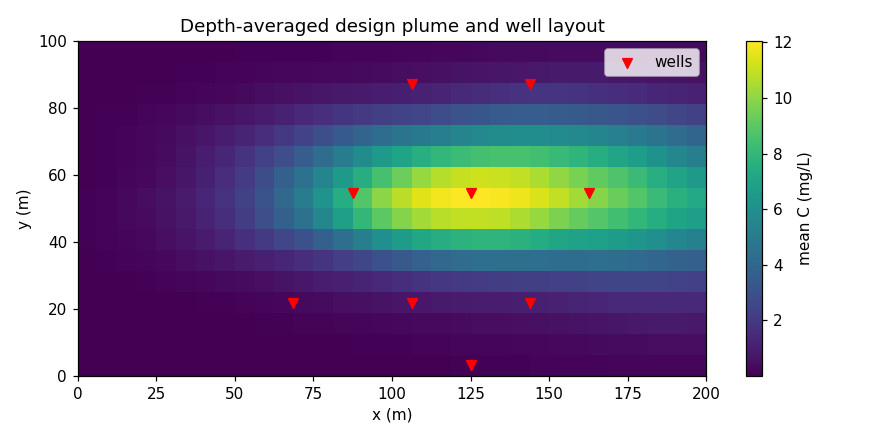
\includegraphics[width=0.86\linewidth]{figs/well_layout_3d.png}
  \caption{Depth-averaged mean concentration of the design plume with the nine
    candidate wells, on the paper preset. Triangles mark the wells in plan view;
    the four the optimizer activates are the ones adjacent to the plume, and in
    the vertical they draw from the $6$\,m screened interval rather than the full
    $20$\,m thickness. The plume is confined to roughly the middle third of the
    thickness at the source and spreads vertically as it travels, which is what
    makes the screen placement matter.}
  \label{fig:3d-layout}
\end{figure}

The paper preset converges to
\[
  \mathbf{q}^* = [12.5,\,12.5,\,12.5,\,12.5,\,0,\,0,\,0,\,0,\,0]\ \mathrm{m^3/d},
  \qquad \textstyle\sum_i q^*_i = 50\ \mathrm{m^3/d},
\]
i.e.\ four of the nine wells at a quarter of the plant capacity each, clustered
around the plume centroid and arranged upstream of the compliance point. Three
properties of this policy are worth stating as measurements rather than as
plausibility arguments:
\begin{itemize}
  \item the four rates are \emph{equal}. The pattern search was free to place
    unequal rates and did so on the coarser \texttt{full} preset
    ($12.89,\,12.70,\,11.91,\,12.50$); at $32\times16\times8$ every active well
    converged to the same $12.5$, which is the signature of a capacity-limited
    rather than a rate-limited design;
  \item the train and test objectives differ by $1.1\times10^{-4}$
    ($547\,605.9$ vs $547\,665.3$), so selecting on $64$ scenarios did not
    overfit the out-of-sample cost --- consistent with the 2D finding that the
    cost of a policy is a robust quantity;
  \item the test reliability is $0.969$ ($124/128$), the mean time to compliance
    is $110.6$\,d, the mean head margin is $10.03$\,m against a $-10$\,m limit,
    and the flow mass ledger closes to machine precision.
\end{itemize}

The comparison that makes the policy legible is against the two trivial designs
(Table~\ref{tab:3d-baselines}). Doing nothing is cheap only because nothing is
cleaned up: $J=314\,330$ with a reliability of $0.000$ and a plume that never
complies within the $3650$\,d horizon. Pumping every well at half capacity is
*cheaper in objective* than the optimized policy ($531\,412$ vs $547\,665$) and
fails more than half the time, with a mean cleanup time of $1996$\,d against
$110.6$\,d. The optimized policy therefore spends about $3\%$ of the objective
to move reliability from $0.453$ to $0.969$ and the cleanup time by a factor of
eighteen. On this geometry the chance constraint, not the pumping cost, is what
moves the design --- the same conclusion the 2D campaign reached, arrived at
from the other side.

\begin{table}[t]
  \centering
  \caption{The optimized paper-preset policy against the two trivial designs, all
  scored on the same $128$ test scenarios. A lower $J$ is not better when the
  policy violates the compliance constraint: the penalty-weighted objective of a
  failing policy understates its cost.}
  \label{tab:3d-baselines}
  \begin{tabular}{@{}lrrrr@{}}
    \toprule
    policy & $J$ & reliability & mean $\tau$ (d) & $\mathrm{CVaR}_{5\%}(G)$ \\
    \midrule
    no pumping & $314\,330$ & $0.000$ & $3650$ & $23.15$ \\
    uniform, half capacity & $531\,412$ & $0.453$ & $1996$ & $2.42$ \\
    optimized $\mathbf{q}^*$ & $547\,665$ & $0.969$ & $110.6$ & $0.10$ \\
    \bottomrule
  \end{tabular}
\end{table}

All six gates of the run pass: retained KL variance $\ge 0.95$,
reproducibility, mass balance $\le 1\%$, test reliability $\ge 1-\alpha-1\%$,
improvement over no pumping, and a no-pump reliability that is not itself
compliant. The optimization took $49$ evaluations and $3$ compass iterations in
$1217$\,s on a four-core laptop at $18.6$\,s per evaluation; the workload is a
sparse LU factorization rather than dense linear algebra, so a GPU buys nothing
and the CPU is the right machine.

\section{Reproducibility across machines}

Because the 3D results rest on a single-file NumPy/SciPy runner rather than on
the 2D optimization stack, the run was repeated on three different machines and
BLAS builds, including one after the 3D and optimization branches were merged
(Table~\ref{tab:3d-repro}). Agreement to five significant figures on the policy
and to $10^{-15}$ on the mass ledger is what allows the result to be quoted as a
number rather than as an anecdote.

\begin{table}[t]
  \centering
  \caption{The paper preset on three machines. The first column is the value the
  preset reports at its first start; the last is the local rerun on the assembled
  tree, which reproduced the policy and the test objective exactly.}
  \label{tab:3d-repro}
  \begin{tabular}{@{}lllrr@{}}
    \toprule
    run & hardware & $\mathbf{q}^*$ (active) & test $J$ & rel. \\
    \midrule
    Colab, partial & 2-core CPU & $4\times12.5$ & --- & --- \\
    laptop, first & 4-core CPU & $4\times12.5$ & $547\,665.31$ & $0.96875$ \\
    laptop, after merge & 4-core CPU & $4\times12.5$ & $547\,665.31$ & $0.96875$ \\
    \bottomrule
  \end{tabular}
\end{table}

\section{What the 3D results do not establish}
\label{sec:3d-not}

The protocol transfers, and that is the claim. Four things are deliberately not
claimed.

\begin{enumerate}
  \item \textbf{The 3D policy is not certified to the standard of
    Chapter~\ref{chap:results_2d}.} Its point-estimate reliability is $0.969$, which
    clears the $0.94$ gate; its Wilson interval at $M=128$ is
    $[0.922,\,0.988]$, which does not. By the reporting rule of
    Chapter~\ref{chap:results_2d} --- certify with the interval, not the point ---
    this is an encouraging but inconclusive certificate, and it needs roughly
    $400$ test scenarios to become the kind of statement the 2D policy earned. That is a compute assertion, not a modelling one: $400$
    scenarios at $18.6$\,s per evaluation is about two hours on one core.
  \item \textbf{No tail is quoted at all.} The 2D campaign showed that
    $\mathrm{CVaR}_{5\%}$ estimated from a few hundred draws moves between draws
    by more than its own standard error. At $M=128$ a $5\%$ tail averages six
    realizations; the number in Table~\ref{tab:3d-baselines} is reported to show
    that the optimized policy's tail is near zero, not as a measurement of it.
  \item \textbf{The discretization is coarse relative to the 2D campaign}:
    $4096$ cells and $1419$ modes against $15\,360$ and $1529$, with a vertical
    resolution of $2.5$\,m and a screened interval of $6$\,m. The vertical
    direction is intentionally coarse, because vertical transport is diffusive at
    $\alpha_{TV}=0.05$\,m and a handful of layers already carries the screen
    contrast, but it means this is a model of partial penetration, not a
    converged solution of a layered aquifer.
  \item \textbf{The physics is deliberately narrower than a site model}: the
    dispersion tensor is diagonal (cross terms omitted), there is no density
    coupling and no NAPL phase, the conductivity is a single log-normal family
    rather than a layered geology, and there is one source and one compliance
    point.
\end{enumerate}

The obvious next step is the one the pipeline was built for and has not yet been
run: the \texttt{paperGPU} preset, which keeps the scenario count and the time
span and refines the grid $2\times$ per axis to $32\,768$ cells, where the batched
torch backend beats sparse LU. Together with layer-resolved conductivity, that
would make the 3D result a statement about a heterogeneous aquifer rather than
about the transferability of a protocol.
.
% Requires: booktabs, amsmath, siunitx (as results_2d.tex does).
% Numbers are verbatim from full3D_colab_run.py --preset paper, whose metrics are
% out3d_colab/run_paper/metrics.json; the solver gates are
% tests/test_fv3d_reference.py and DOCS/3D_results.md.

\label{sec:results-3d}
\section{What changes in three dimensions}

The two-dimensional campaign treats a well as a line source that spans the whole
thickness of the aquifer. A real screen does not: it is a few metres of slotted
casing placed at a chosen depth, and the water it captures comes preferentially
from the layers it crosses. That is not a cosmetic difference. Partial
penetration creates vertical head gradients, so the flow field is no longer a
depth average; vertical anisotropy decides how much of the plume a screen can
see; and the same total pumping rate can be a good or a useless design depending
on where along the vertical the screen sits.

This chapter asks a narrower question than the 2D campaign: does the protocol of
Chapter~\ref{chap:results_2d} --- sample-average objective, CVaR chance constraint,
derivative-free search, out-of-sample certificate --- survive the change of
dimension, and what does it cost? It is not an attempt to model a field site,
and Section~\ref{sec:3d-not} is explicit about what it therefore cannot claim.

\section{Model, discretization, and the reference solver}

The 3D model keeps the same governing equations as
Chapter~\ref{chap:formulation} and adds only the vertical direction:
\begin{align}
  -\nabla\cdot\bigl(K\nabla h\bigr) &= W, \\
  \frac{\partial(\phi R C)}{\partial t} + \nabla\cdot(\mathbf{v}C)
  - \nabla\cdot(\mathbf{D}\nabla C) &= S,
\end{align}
with $K$ log-normal, separable in the three axes and truncated at $1419$
Karhunen--Lo\`eve modes ($95\%$ of the variance, $\sigma=0.5$,
$\ell_x=\ell_y=20$\,m, $\ell_z=6$\,m), $K_v=0.1\,K_h$
\citep{bear1972,li2020fourier}. Flow uses a seven-point two-point-flux
approximation with harmonic face conductances and a sparse LU factorization;
transport is implicit Euler with first-order upwinding and the diagonal part of
the Bear dispersion tensor ($\alpha_L=5$, $\alpha_{TH}=0.5$,
$\alpha_{TV}=0.05$\,m). Wells are partially penetrating, with a Gaussian
footprint in the horizontal plane and a screened interval covering the middle
$30\%$ of the thickness.

The discretization is verified before anything is optimized, and the gates were
chosen to test the \emph{extension}, not to re-test the scheme: agreement with the 2D
code is the claim, and an analytical 1D shape gate would test the upwinding that
both codes share.

\begin{table}[t]
  \centering
  \caption{Gates on the 3D solver, all asserted in
    \texttt{tests/test\_fv3d\_reference.py}. The fourth row is the decisive one:
    an extruded column must reproduce the trusted 2D column to machine
    precision, which it does, so the 3D flow and transport agree with 2D physics
    rather than merely resembling it.}
  \label{tab:3d-gates}
  \begin{tabular}{@{}lll@{}}
    \toprule
    property & measured & gate \\
    \midrule
    seepage velocity $K\nabla h/\phi$ & exact & $10^{-12}$ \\
    head invariant across $y,z$ & exact & $10^{-12}$ \\
    Thiem shape, fully penetrating well & $8.1\times10^{-3}$ & $10^{-2}$ \\
    \textbf{3D column vs 2D column (extrusion)} & $\mathbf{1.9\times10^{-13}}$ & $10^{-9}$ \\
    advection front speed (advective limit) & $1.2\%$ low, $0.8\,\Delta x$ lag & $2\%$ \\
    breakthrough variance $\Rightarrow D_{\text{eff}}$ & $0.24$--$0.31\,D$ & $20\%$ \\
    mass ledger closure (rel.) & $10^{-15}$ & $10^{-9}$ \\
    \bottomrule
  \end{tabular}
\end{table}

Table~\ref{tab:3d-gates} lists what was measured. Two entries deserve comment.
The front travels at the pore velocity to within $1.2\%$, short by a constant
$0.8\Delta x$: that is first-order upwinding, not a defect, and it is why the
gate is stated with the lag rather than against the exact front position. The
breakthrough variance implies an effective dispersion of
$0.24/0.29/0.31$ of $\alpha_L v$ at $t=1000/2000/3000$\,d, approaching the
analytical value from below: the numerical profile is \emph{steeper} than the
analytical one at early time, i.e. the scheme under-disperses rather than
over-smears.

There is deliberately no Ogata--Banks shape gate
\citep{ogata1961solution}. The analytical solution is a continuous
Dirichlet-source step, and comparing it against a finite inlet profile gives a
relative $L^2$ error of $0.32$ that decays to $0.13$ as the profile develops ---
a statement about truncation error, not about three dimensions. The trustworthy
gate for a second implementation is agreement with the first, and that is what
row four of the table provides.

\section{The paper preset}

The 3D campaign runs on a $200\times100\times20$\,m aquifer discretized on
$32\times16\times8$ cells ($4096$ unknowns, $6.25\times6.25\times2.5$\,m),
$64$ training and $128$ test scenarios, and the same nine candidate wells, cost
model, penalty weights ($\rho_g=\rho_h=10^{6}$), $5\%$ concentration chance
constraint and $1\%$ head constraint as the 2D runs. Table~\ref{tab:3d-presets}
places it beside the two smaller presets that were used to debug the pipeline.

\begin{table}[t]
  \centering
  \caption{Presets of the 3D pipeline. The smoke preset is degenerate on purpose
  --- the source is weak enough that the unpumped plume already complies, so
  $\mathbf{q}^*=\mathbf{0}$ is the correct answer there and it is not a
  candidate for a result.}
  \label{tab:3d-presets}
  \begin{tabular}{@{}lrrrrl@{}}
    \toprule
    preset & cells & $n_{KL}$ & scenarios (tr/te) & wells & outcome \\
    \midrule
    smoke & $12\cdot6\cdot3=216$ & 164 & 6 / 12 & 4 & degenerate, $\mathbf{q}^*=\mathbf{0}$ \\
    full & $24\cdot12\cdot6=1728$ & 819 & 24 / 48 & 6 & 4 active wells, test rel.\ $0.979$ \\
    paper & $32\cdot16\cdot8=4096$ & 1419 & 64 / 128 & 9 & 4 active wells, test rel.\ $0.969$ \\
    \bottomrule
  \end{tabular}
\end{table}

\begin{figure}[t]
  \centering
  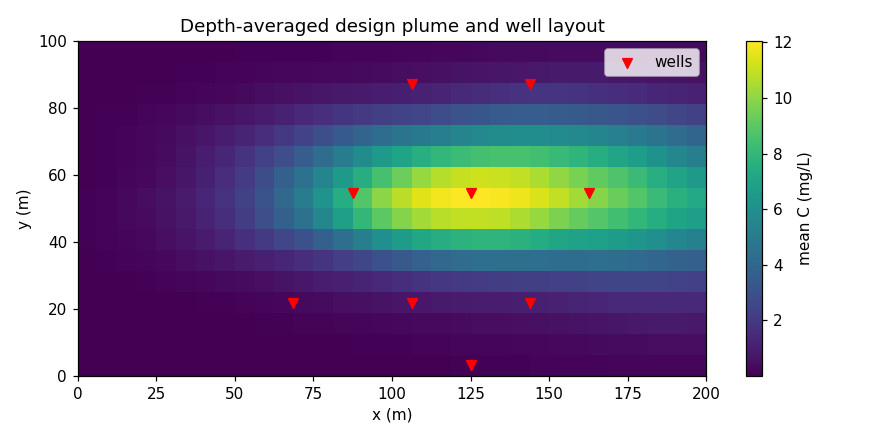
\includegraphics[width=0.86\linewidth]{figs/well_layout_3d.png}
  \caption{Depth-averaged mean concentration of the design plume with the nine
    candidate wells, on the paper preset. Triangles mark the wells in plan view;
    the four the optimizer activates are the ones adjacent to the plume, and in
    the vertical they draw from the $6$\,m screened interval rather than the full
    $20$\,m thickness. The plume is confined to roughly the middle third of the
    thickness at the source and spreads vertically as it travels, which is what
    makes the screen placement matter.}
  \label{fig:3d-layout}
\end{figure}

The paper preset converges to
\[
  \mathbf{q}^* = [12.5,\,12.5,\,12.5,\,12.5,\,0,\,0,\,0,\,0,\,0]\ \mathrm{m^3/d},
  \qquad \textstyle\sum_i q^*_i = 50\ \mathrm{m^3/d},
\]
i.e.\ four of the nine wells at a quarter of the plant capacity each, clustered
around the plume centroid and arranged upstream of the compliance point. Three
properties of this policy are worth stating as measurements rather than as
plausibility arguments:
\begin{itemize}
  \item the four rates are \emph{equal}. The pattern search was free to place
    unequal rates and did so on the coarser \texttt{full} preset
    ($12.89,\,12.70,\,11.91,\,12.50$); at $32\times16\times8$ every active well
    converged to the same $12.5$, which is the signature of a capacity-limited
    rather than a rate-limited design;
  \item the train and test objectives differ by $1.1\times10^{-4}$
    ($547\,605.9$ vs $547\,665.3$), so selecting on $64$ scenarios did not
    overfit the out-of-sample cost --- consistent with the 2D finding that the
    cost of a policy is a robust quantity;
  \item the test reliability is $0.969$ ($124/128$), the mean time to compliance
    is $110.6$\,d, the mean head margin is $10.03$\,m against a $-10$\,m limit,
    and the flow mass ledger closes to machine precision.
\end{itemize}

The comparison that makes the policy legible is against the two trivial designs
(Table~\ref{tab:3d-baselines}). Doing nothing is cheap only because nothing is
cleaned up: $J=314\,330$ with a reliability of $0.000$ and a plume that never
complies within the $3650$\,d horizon. Pumping every well at half capacity is
*cheaper in objective* than the optimized policy ($531\,412$ vs $547\,665$) and
fails more than half the time, with a mean cleanup time of $1996$\,d against
$110.6$\,d. The optimized policy therefore spends about $3\%$ of the objective
to move reliability from $0.453$ to $0.969$ and the cleanup time by a factor of
eighteen. On this geometry the chance constraint, not the pumping cost, is what
moves the design --- the same conclusion the 2D campaign reached, arrived at
from the other side.

\begin{table}[t]
  \centering
  \caption{The optimized paper-preset policy against the two trivial designs, all
  scored on the same $128$ test scenarios. A lower $J$ is not better when the
  policy violates the compliance constraint: the penalty-weighted objective of a
  failing policy understates its cost.}
  \label{tab:3d-baselines}
  \begin{tabular}{@{}lrrrr@{}}
    \toprule
    policy & $J$ & reliability & mean $\tau$ (d) & $\mathrm{CVaR}_{5\%}(G)$ \\
    \midrule
    no pumping & $314\,330$ & $0.000$ & $3650$ & $23.15$ \\
    uniform, half capacity & $531\,412$ & $0.453$ & $1996$ & $2.42$ \\
    optimized $\mathbf{q}^*$ & $547\,665$ & $0.969$ & $110.6$ & $0.10$ \\
    \bottomrule
  \end{tabular}
\end{table}

All six gates of the run pass: retained KL variance $\ge 0.95$,
reproducibility, mass balance $\le 1\%$, test reliability $\ge 1-\alpha-1\%$,
improvement over no pumping, and a no-pump reliability that is not itself
compliant. The optimization took $49$ evaluations and $3$ compass iterations in
$1217$\,s on a four-core laptop at $18.6$\,s per evaluation; the workload is a
sparse LU factorization rather than dense linear algebra, so a GPU buys nothing
and the CPU is the right machine.

\section{Reproducibility across machines}

Because the 3D results rest on a single-file NumPy/SciPy runner rather than on
the 2D optimization stack, the run was repeated on three different machines and
BLAS builds, including one after the 3D and optimization branches were merged
(Table~\ref{tab:3d-repro}). Agreement to five significant figures on the policy
and to $10^{-15}$ on the mass ledger is what allows the result to be quoted as a
number rather than as an anecdote.

\begin{table}[t]
  \centering
  \caption{The paper preset on three machines. The first column is the value the
  preset reports at its first start; the last is the local rerun on the assembled
  tree, which reproduced the policy and the test objective exactly.}
  \label{tab:3d-repro}
  \begin{tabular}{@{}lllrr@{}}
    \toprule
    run & hardware & $\mathbf{q}^*$ (active) & test $J$ & rel. \\
    \midrule
    Colab, partial & 2-core CPU & $4\times12.5$ & --- & --- \\
    laptop, first & 4-core CPU & $4\times12.5$ & $547\,665.31$ & $0.96875$ \\
    laptop, after merge & 4-core CPU & $4\times12.5$ & $547\,665.31$ & $0.96875$ \\
    \bottomrule
  \end{tabular}
\end{table}

\section{What the 3D results do not establish}
\label{sec:3d-not}

The protocol transfers, and that is the claim. Four things are deliberately not
claimed.

\begin{enumerate}
  \item \textbf{The 3D policy is not certified to the standard of
    Chapter~\ref{chap:results_2d}.} Its point-estimate reliability is $0.969$, which
    clears the $0.94$ gate; its Wilson interval at $M=128$ is
    $[0.922,\,0.988]$, which does not. By the reporting rule of
    Chapter~\ref{chap:results_2d} --- certify with the interval, not the point ---
    this is an encouraging but inconclusive certificate, and it needs roughly
    $400$ test scenarios to become the kind of statement the 2D policy earned. That is a compute assertion, not a modelling one: $400$
    scenarios at $18.6$\,s per evaluation is about two hours on one core.
  \item \textbf{No tail is quoted at all.} The 2D campaign showed that
    $\mathrm{CVaR}_{5\%}$ estimated from a few hundred draws moves between draws
    by more than its own standard error. At $M=128$ a $5\%$ tail averages six
    realizations; the number in Table~\ref{tab:3d-baselines} is reported to show
    that the optimized policy's tail is near zero, not as a measurement of it.
  \item \textbf{The discretization is coarse relative to the 2D campaign}:
    $4096$ cells and $1419$ modes against $15\,360$ and $1529$, with a vertical
    resolution of $2.5$\,m and a screened interval of $6$\,m. The vertical
    direction is intentionally coarse, because vertical transport is diffusive at
    $\alpha_{TV}=0.05$\,m and a handful of layers already carries the screen
    contrast, but it means this is a model of partial penetration, not a
    converged solution of a layered aquifer.
  \item \textbf{The physics is deliberately narrower than a site model}: the
    dispersion tensor is diagonal (cross terms omitted), there is no density
    coupling and no NAPL phase, the conductivity is a single log-normal family
    rather than a layered geology, and there is one source and one compliance
    point.
\end{enumerate}

The obvious next step is the one the pipeline was built for and has not yet been
run: the \texttt{paperGPU} preset, which keeps the scenario count and the time
span and refines the grid $2\times$ per axis to $32\,768$ cells, where the batched
torch backend beats sparse LU. Together with layer-resolved conductivity, that
would make the 3D result a statement about a heterogeneous aquifer rather than
about the transferability of a protocol.
.
% Requires: booktabs, amsmath, siunitx (as results_2d.tex does).
% Numbers are verbatim from full3D_colab_run.py --preset paper, whose metrics are
% out3d_colab/run_paper/metrics.json; the solver gates are
% tests/test_fv3d_reference.py and DOCS/3D_results.md.

\label{sec:results-3d}
\section{What changes in three dimensions}

The two-dimensional campaign treats a well as a line source that spans the whole
thickness of the aquifer. A real screen does not: it is a few metres of slotted
casing placed at a chosen depth, and the water it captures comes preferentially
from the layers it crosses. That is not a cosmetic difference. Partial
penetration creates vertical head gradients, so the flow field is no longer a
depth average; vertical anisotropy decides how much of the plume a screen can
see; and the same total pumping rate can be a good or a useless design depending
on where along the vertical the screen sits.

This chapter asks a narrower question than the 2D campaign: does the protocol of
Chapter~\ref{chap:results_2d} --- sample-average objective, CVaR chance constraint,
derivative-free search, out-of-sample certificate --- survive the change of
dimension, and what does it cost? It is not an attempt to model a field site,
and Section~\ref{sec:3d-not} is explicit about what it therefore cannot claim.

\section{Model, discretization, and the reference solver}

The 3D model keeps the same governing equations as
Chapter~\ref{chap:formulation} and adds only the vertical direction:
\begin{align}
  -\nabla\cdot\bigl(K\nabla h\bigr) &= W, \\
  \frac{\partial(\phi R C)}{\partial t} + \nabla\cdot(\mathbf{v}C)
  - \nabla\cdot(\mathbf{D}\nabla C) &= S,
\end{align}
with $K$ log-normal, separable in the three axes and truncated at $1419$
Karhunen--Lo\`eve modes ($95\%$ of the variance, $\sigma=0.5$,
$\ell_x=\ell_y=20$\,m, $\ell_z=6$\,m), $K_v=0.1\,K_h$
\citep{bear1972,li2020fourier}. Flow uses a seven-point two-point-flux
approximation with harmonic face conductances and a sparse LU factorization;
transport is implicit Euler with first-order upwinding and the diagonal part of
the Bear dispersion tensor ($\alpha_L=5$, $\alpha_{TH}=0.5$,
$\alpha_{TV}=0.05$\,m). Wells are partially penetrating, with a Gaussian
footprint in the horizontal plane and a screened interval covering the middle
$30\%$ of the thickness.

The discretization is verified before anything is optimized, and the gates were
chosen to test the \emph{extension}, not to re-test the scheme: agreement with the 2D
code is the claim, and an analytical 1D shape gate would test the upwinding that
both codes share.

\begin{table}[t]
  \centering
  \caption{Gates on the 3D solver, all asserted in
    \texttt{tests/test\_fv3d\_reference.py}. The fourth row is the decisive one:
    an extruded column must reproduce the trusted 2D column to machine
    precision, which it does, so the 3D flow and transport agree with 2D physics
    rather than merely resembling it.}
  \label{tab:3d-gates}
  \begin{tabular}{@{}lll@{}}
    \toprule
    property & measured & gate \\
    \midrule
    seepage velocity $K\nabla h/\phi$ & exact & $10^{-12}$ \\
    head invariant across $y,z$ & exact & $10^{-12}$ \\
    Thiem shape, fully penetrating well & $8.1\times10^{-3}$ & $10^{-2}$ \\
    \textbf{3D column vs 2D column (extrusion)} & $\mathbf{1.9\times10^{-13}}$ & $10^{-9}$ \\
    advection front speed (advective limit) & $1.2\%$ low, $0.8\,\Delta x$ lag & $2\%$ \\
    breakthrough variance $\Rightarrow D_{\text{eff}}$ & $0.24$--$0.31\,D$ & $20\%$ \\
    mass ledger closure (rel.) & $10^{-15}$ & $10^{-9}$ \\
    \bottomrule
  \end{tabular}
\end{table}

Table~\ref{tab:3d-gates} lists what was measured. Two entries deserve comment.
The front travels at the pore velocity to within $1.2\%$, short by a constant
$0.8\Delta x$: that is first-order upwinding, not a defect, and it is why the
gate is stated with the lag rather than against the exact front position. The
breakthrough variance implies an effective dispersion of
$0.24/0.29/0.31$ of $\alpha_L v$ at $t=1000/2000/3000$\,d, approaching the
analytical value from below: the numerical profile is \emph{steeper} than the
analytical one at early time, i.e. the scheme under-disperses rather than
over-smears.

There is deliberately no Ogata--Banks shape gate
\citep{ogata1961solution}. The analytical solution is a continuous
Dirichlet-source step, and comparing it against a finite inlet profile gives a
relative $L^2$ error of $0.32$ that decays to $0.13$ as the profile develops ---
a statement about truncation error, not about three dimensions. The trustworthy
gate for a second implementation is agreement with the first, and that is what
row four of the table provides.

\section{The paper preset}

The 3D campaign runs on a $200\times100\times20$\,m aquifer discretized on
$32\times16\times8$ cells ($4096$ unknowns, $6.25\times6.25\times2.5$\,m),
$64$ training and $128$ test scenarios, and the same nine candidate wells, cost
model, penalty weights ($\rho_g=\rho_h=10^{6}$), $5\%$ concentration chance
constraint and $1\%$ head constraint as the 2D runs. Table~\ref{tab:3d-presets}
places it beside the two smaller presets that were used to debug the pipeline.

\begin{table}[t]
  \centering
  \caption{Presets of the 3D pipeline. The smoke preset is degenerate on purpose
  --- the source is weak enough that the unpumped plume already complies, so
  $\mathbf{q}^*=\mathbf{0}$ is the correct answer there and it is not a
  candidate for a result.}
  \label{tab:3d-presets}
  \begin{tabular}{@{}lrrrrl@{}}
    \toprule
    preset & cells & $n_{KL}$ & scenarios (tr/te) & wells & outcome \\
    \midrule
    smoke & $12\cdot6\cdot3=216$ & 164 & 6 / 12 & 4 & degenerate, $\mathbf{q}^*=\mathbf{0}$ \\
    full & $24\cdot12\cdot6=1728$ & 819 & 24 / 48 & 6 & 4 active wells, test rel.\ $0.979$ \\
    paper & $32\cdot16\cdot8=4096$ & 1419 & 64 / 128 & 9 & 4 active wells, test rel.\ $0.969$ \\
    \bottomrule
  \end{tabular}
\end{table}

\begin{figure}[t]
  \centering
  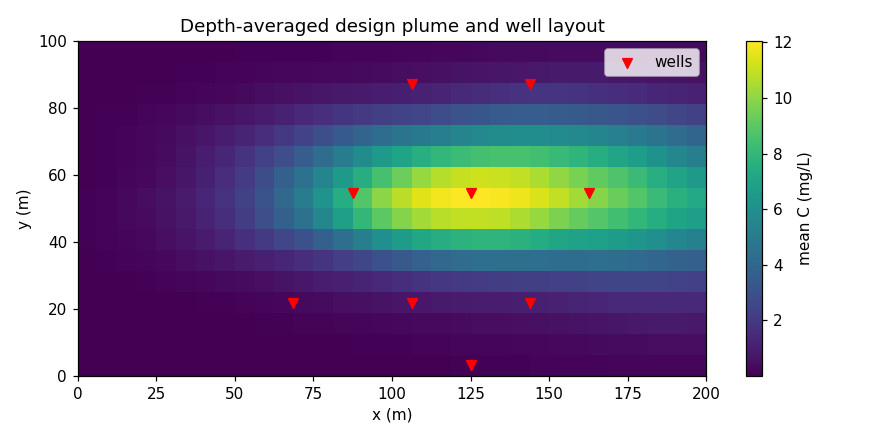
\includegraphics[width=0.86\linewidth]{figs/well_layout_3d.png}
  \caption{Depth-averaged mean concentration of the design plume with the nine
    candidate wells, on the paper preset. Triangles mark the wells in plan view;
    the four the optimizer activates are the ones adjacent to the plume, and in
    the vertical they draw from the $6$\,m screened interval rather than the full
    $20$\,m thickness. The plume is confined to roughly the middle third of the
    thickness at the source and spreads vertically as it travels, which is what
    makes the screen placement matter.}
  \label{fig:3d-layout}
\end{figure}

The paper preset converges to
\[
  \mathbf{q}^* = [12.5,\,12.5,\,12.5,\,12.5,\,0,\,0,\,0,\,0,\,0]\ \mathrm{m^3/d},
  \qquad \textstyle\sum_i q^*_i = 50\ \mathrm{m^3/d},
\]
i.e.\ four of the nine wells at a quarter of the plant capacity each, clustered
around the plume centroid and arranged upstream of the compliance point. Three
properties of this policy are worth stating as measurements rather than as
plausibility arguments:
\begin{itemize}
  \item the four rates are \emph{equal}. The pattern search was free to place
    unequal rates and did so on the coarser \texttt{full} preset
    ($12.89,\,12.70,\,11.91,\,12.50$); at $32\times16\times8$ every active well
    converged to the same $12.5$, which is the signature of a capacity-limited
    rather than a rate-limited design;
  \item the train and test objectives differ by $1.1\times10^{-4}$
    ($547\,605.9$ vs $547\,665.3$), so selecting on $64$ scenarios did not
    overfit the out-of-sample cost --- consistent with the 2D finding that the
    cost of a policy is a robust quantity;
  \item the test reliability is $0.969$ ($124/128$), the mean time to compliance
    is $110.6$\,d, the mean head margin is $10.03$\,m against a $-10$\,m limit,
    and the flow mass ledger closes to machine precision.
\end{itemize}

The comparison that makes the policy legible is against the two trivial designs
(Table~\ref{tab:3d-baselines}). Doing nothing is cheap only because nothing is
cleaned up: $J=314\,330$ with a reliability of $0.000$ and a plume that never
complies within the $3650$\,d horizon. Pumping every well at half capacity is
*cheaper in objective* than the optimized policy ($531\,412$ vs $547\,665$) and
fails more than half the time, with a mean cleanup time of $1996$\,d against
$110.6$\,d. The optimized policy therefore spends about $3\%$ of the objective
to move reliability from $0.453$ to $0.969$ and the cleanup time by a factor of
eighteen. On this geometry the chance constraint, not the pumping cost, is what
moves the design --- the same conclusion the 2D campaign reached, arrived at
from the other side.

\begin{table}[t]
  \centering
  \caption{The optimized paper-preset policy against the two trivial designs, all
  scored on the same $128$ test scenarios. A lower $J$ is not better when the
  policy violates the compliance constraint: the penalty-weighted objective of a
  failing policy understates its cost.}
  \label{tab:3d-baselines}
  \begin{tabular}{@{}lrrrr@{}}
    \toprule
    policy & $J$ & reliability & mean $\tau$ (d) & $\mathrm{CVaR}_{5\%}(G)$ \\
    \midrule
    no pumping & $314\,330$ & $0.000$ & $3650$ & $23.15$ \\
    uniform, half capacity & $531\,412$ & $0.453$ & $1996$ & $2.42$ \\
    optimized $\mathbf{q}^*$ & $547\,665$ & $0.969$ & $110.6$ & $0.10$ \\
    \bottomrule
  \end{tabular}
\end{table}

All six gates of the run pass: retained KL variance $\ge 0.95$,
reproducibility, mass balance $\le 1\%$, test reliability $\ge 1-\alpha-1\%$,
improvement over no pumping, and a no-pump reliability that is not itself
compliant. The optimization took $49$ evaluations and $3$ compass iterations in
$1217$\,s on a four-core laptop at $18.6$\,s per evaluation; the workload is a
sparse LU factorization rather than dense linear algebra, so a GPU buys nothing
and the CPU is the right machine.

\section{Reproducibility across machines}

Because the 3D results rest on a single-file NumPy/SciPy runner rather than on
the 2D optimization stack, the run was repeated on three different machines and
BLAS builds, including one after the 3D and optimization branches were merged
(Table~\ref{tab:3d-repro}). Agreement to five significant figures on the policy
and to $10^{-15}$ on the mass ledger is what allows the result to be quoted as a
number rather than as an anecdote.

\begin{table}[t]
  \centering
  \caption{The paper preset on three machines. The first column is the value the
  preset reports at its first start; the last is the local rerun on the assembled
  tree, which reproduced the policy and the test objective exactly.}
  \label{tab:3d-repro}
  \begin{tabular}{@{}lllrr@{}}
    \toprule
    run & hardware & $\mathbf{q}^*$ (active) & test $J$ & rel. \\
    \midrule
    Colab, partial & 2-core CPU & $4\times12.5$ & --- & --- \\
    laptop, first & 4-core CPU & $4\times12.5$ & $547\,665.31$ & $0.96875$ \\
    laptop, after merge & 4-core CPU & $4\times12.5$ & $547\,665.31$ & $0.96875$ \\
    \bottomrule
  \end{tabular}
\end{table}

\section{What the 3D results do not establish}
\label{sec:3d-not}

The protocol transfers, and that is the claim. Four things are deliberately not
claimed.

\begin{enumerate}
  \item \textbf{The 3D policy is not certified to the standard of
    Chapter~\ref{chap:results_2d}.} Its point-estimate reliability is $0.969$, which
    clears the $0.94$ gate; its Wilson interval at $M=128$ is
    $[0.922,\,0.988]$, which does not. By the reporting rule of
    Chapter~\ref{chap:results_2d} --- certify with the interval, not the point ---
    this is an encouraging but inconclusive certificate, and it needs roughly
    $400$ test scenarios to become the kind of statement the 2D policy earned. That is a compute assertion, not a modelling one: $400$
    scenarios at $18.6$\,s per evaluation is about two hours on one core.
  \item \textbf{No tail is quoted at all.} The 2D campaign showed that
    $\mathrm{CVaR}_{5\%}$ estimated from a few hundred draws moves between draws
    by more than its own standard error. At $M=128$ a $5\%$ tail averages six
    realizations; the number in Table~\ref{tab:3d-baselines} is reported to show
    that the optimized policy's tail is near zero, not as a measurement of it.
  \item \textbf{The discretization is coarse relative to the 2D campaign}:
    $4096$ cells and $1419$ modes against $15\,360$ and $1529$, with a vertical
    resolution of $2.5$\,m and a screened interval of $6$\,m. The vertical
    direction is intentionally coarse, because vertical transport is diffusive at
    $\alpha_{TV}=0.05$\,m and a handful of layers already carries the screen
    contrast, but it means this is a model of partial penetration, not a
    converged solution of a layered aquifer.
  \item \textbf{The physics is deliberately narrower than a site model}: the
    dispersion tensor is diagonal (cross terms omitted), there is no density
    coupling and no NAPL phase, the conductivity is a single log-normal family
    rather than a layered geology, and there is one source and one compliance
    point.
\end{enumerate}

The obvious next step is the one the pipeline was built for and has not yet been
run: the \texttt{paperGPU} preset, which keeps the scenario count and the time
span and refines the grid $2\times$ per axis to $32\,768$ cells, where the batched
torch backend beats sparse LU. Together with layer-resolved conductivity, that
would make the 3D result a statement about a heterogeneous aquifer rather than
about the transferability of a protocol.
